\section*{(10\textordfeminine\ aula) --- Problemas com a Mecânica Clássica e Dualidade Onda-Partícula (cap. 3)}

\subsection*{Problemas com a Mecânica Clássica}

Vimos na 1\textordfeminine\ aula um apanhado dos problemas que apontavam para a inadequação da Mecânica Clássica para descrever certos resultados experimentais.

\textbf{Física Atômica:}
\begin{enumerate}
    \item[(i)] Por que os átomos, quando excitados, só emitem radiação EM em certas frequências bem definidas? (problema do espectro atômico)
    \item[(ii)] Por que os elétrons dos átomos, atraídos pelo núcleo positivo, não emitem continuamente radiação e colapsam no interior do núcleo? (problema da estabilidade da matéria)
\end{enumerate}

Esses problemas não podem ser solucionados caso se insista em descrever o movimento dos elétrons de maneira clássica, através de uma trajetória $\vec{r}(t)$ que obedeça à Eq. de Newton, $\vec{F} = m\ddot{\vec{r}}$.

A evidência mais concreta da necessidade de se usar outro tipo de descrição para a dinâmica de elétrons veio da experiência de Davisson e Germer ($\sim 1925$), que mostrou que elétrons se \textbf{difratavam} quando incidentes em uma superfície metálica. Vamos discutir essa experiência (ou uma versão idealizada dela) na aula de hoje.

Com respeito à \textbf{radiação EM}, os problemas que não tinham explicação clássica (em termos de uma onda dos campos $\vec{E}$ e $\vec{B}$) eram (entre outros):

\begin{enumerate}
    \item[(i)] Problema da radiação emitida por um corpo à temperatura $T$
    \item[(ii)] Problema do efeito fotoelétrico
    \item[(iii)] Problema do espalhamento Compton
\end{enumerate}

Esses três fenômenos evidenciavam que a radiação EM carrega energia e momentum em ``pacotes'', relacionados à frequência e ao comprimento de onda por
\begin{equation}
    E = h\nu \qquad \text{e} \qquad p = \frac{h}{\lambda}
\label{eq:aula10_E_p_pacotes}
\end{equation}

O capítulo 3 do livro é dedicado a descrever um experimento idealizado que ilustra como a natureza \textbf{corpuscular} e \textbf{ondulatória} dos elétrons, fótons, prótons, átomos, etc., pode se manifestar simultaneamente.

\subsection*{Partícula vs. Onda}

Classicamente, um objeto da natureza é classificado ou como uma \textbf{PARTÍCULA} (localizado espacialmente, carrega energia e momentum), à qual se pode associar uma posição $\vec{r}(t)$ e uma velocidade $\vec{v}(t)$ em qualquer instante de tempo, ou como uma \textbf{ONDA} (perturbação que se estende por todo o espaço), à qual se pode associar um campo $\Psi(\vec{r}, t)$.

\textbf{Ondas planas} são um tipo de perturbação descrita, por exemplo, pelo campo
\begin{equation}
    \Psi(x,t) = A\cos(kx - \omega t)
\label{eq:aula10_onda_plana_1d}
\end{equation}
ou, em 3D,
\begin{equation}
    \Psi(\vec{r}, t) = A\cos(\vec{k}\cdot\vec{r} - \omega t)
\label{eq:aula10_onda_plana_3d}
\end{equation}

$k = 2\pi/\lambda$ é o vetor de onda, $\lambda$ é o comprimento de onda, $\omega = 2\pi\nu$ é a frequência angular e $\nu = 1/T$ é a frequência (inverso do período).

Em qualquer tempo, o valor de $\Psi$ em pontos espaçados de $\lambda$ é o mesmo (no caso 3D, o valor de $\Psi$ em planos perpendiculares ao vetor $\vec{k}$ e espaçados de $\lambda = 2\pi/|\vec{k}|$ é o mesmo, daí o nome ``onda plana''). O valor de $\Psi$ em um dado ponto $\vec{r}$ se repete a cada $T$ segundos.

\subsection*{Interferência: Experimento de Dupla Fenda}

Ondas planas experimentam \textbf{INTERFERÊNCIA} quando forçadas a passar simultaneamente por 2 orifícios separados por uma distância $d \sim \lambda$.

\begin{center}
\begin{tikzpicture}[scale=1]

    \foreach \x in {0,0.3,0.6}
        \draw[thick] (\x,-1.3) -- (\x,1.3);
    \draw[->, thick] (-0.9,0) -- (-0.1,0) node[midway, above] {$\vec{k}$};


    \draw[thick] (1.3,-1.6) -- (1.3,-0.15);
    \draw[thick] (1.3,0.15) -- (1.3,1.6);
    \node[left] at (1.25,0.4) {$S_1$};
    \node[left] at (1.25,-0.4) {$S_2$};
    \draw[<->] (1.0,-0.15) -- (1.0,0.15);
    \node[left] at (0.95,0) {$d$};


    \draw[thick] (5.2,-1.8) -- (5.2,1.8) node[above] {anteparo};


    \draw[->] (1.3,0.3) -- (5.2,1.3);
    \draw[->] (1.3,-0.3) -- (5.2,1.3);


    \draw[domain=-1.6:1.6, smooth, variable=\y, samples=80]
        plot ({5.2+0.45*((cos(((\y-1.3)*220) ))*(exp(-((\y-1.3)*(\y-1.3))*0.45)) }, \y);

    \draw[<->] (5.7,0.15) -- (5.7,1.3);
    \node[right] at (5.9,0.75) {$\dfrac{\lambda D}{d}$};

    \draw[<->] (1.3,-2.1) -- (5.2,-2.1);
    \node[below] at (3.25,-2.1) {$D$};
\end{tikzpicture}
\end{center}

Você já deve ter visto esse experimento com luz. As franjas claras e escuras são consequência da soma do sinal que passou por $S_1$ com o sinal que passou por $S_2$; como eles devem percorrer distâncias diferentes para chegar ao anteparo, em alguns pontos $\Psi_1 + \Psi_2 = 0$ e em outros $\Psi_1 + \Psi_2 = 2\Psi_1$. Como o sinal luminoso é proporcional ao \textbf{QUADRADO} do valor de $\Psi$ no ponto, se observam as franjas características.

Esse fenômeno, tipicamente ondulatório, permite concluir que a radiação EM deve ser descrita como \textbf{ONDA}.

\subsection*{Mas e os fótons do efeito fotoelétrico?}

Se você diminuir a intensidade da radiação incidente nos orifícios, você vê que a radiação chega ao anteparo em ``pacotes''. É irresistível imaginar que esses pacotes são partículas e, portanto, não deveriam exibir o padrão de interferência.

\textbf{No entanto}, mesmo chegando na forma de partícula, os fótons constroem o padrão de interferência quando os deixamos se acumular no anteparo.

\textbf{Conclusão:} A \textbf{ONDA} EM de alguma maneira governa a distribuição de suas \textbf{PARTÍCULAS} associadas. É possível determinar como a onda irá se distribuir no anteparo, mas é impossível saber onde os fótons irão aparecer. De algum modo, $|\vec{E}(\vec{r},t)|^2$ está relacionado à \textbf{PROBABILIDADE} de encontrar um fóton em $\vec{r}$ no instante $t$.

A isso se chama \textbf{dualidade onda-partícula}. A razão pela qual a natureza-partícula da radiação EM demorou tanto tempo para ser percebida está no fato de que, para intensidades encontradas no dia a dia, o número de fótons é tão grande que não há como perceber que eles chegam individualmente.

\fbox{\parbox{0.92\textwidth}{
\textbf{Exemplo:} Lâmpada de 100 W a 10 m de distância.

\begin{center}
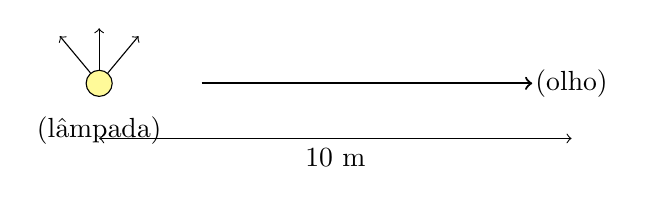
\begin{tikzpicture}[scale=1]
    \node[circle, draw, fill=yellow!40] (lamp) at (0,0) {};
    \draw[->] (lamp) -- ++(-0.5,0.6);
    \draw[->] (lamp) -- ++(0,0.7);
    \draw[->] (lamp) -- ++(0.5,0.6);
    \node[below] at (0,-0.3) {(lâmpada)};
    \draw[->, thick] (1.3,0) -- (5.5,0);
    \node at (6,0) {(olho)};
    \draw[<->] (0,-0.7) -- (6,-0.7);
    \node[below] at (3,-0.7) {10 m};
\end{tikzpicture}
\end{center}

A intensidade que chega ao olho é
\begin{equation}
    I = \frac{100\,\text{W}}{4\pi(10\,\text{m})^2} = 7{,}96\times10^{-2}\ \text{J}/\text{m}^2\text{s}
\label{eq:aula10_intensidade_lampada}
\end{equation}

O raio da pupila é $r \sim 1\,\text{mm}$, então o número de fótons (suponha luz amarela, $\lambda = 5890\ \text{\AA}$) que chega por segundo na retina é dado por
\begin{equation}
    \underbrace{\left(7{,}96\times10^{-2}\ \frac{\text{W}}{\text{m}^2}\right)\left(\pi(1\,\text{mm})^2\right)}_{\text{área da pupila}} = N \underbrace{\left(\frac{hc}{\lambda}\right)}_{\substack{\text{energia de}\\ \text{cada fóton}}}
\label{eq:aula10_fotons_retina}
\end{equation}
\begin{equation}
    \boxed{N = 7{,}4\times10^{11}\ \text{fótons por segundo!}}
\label{eq:aula10_N_fotons}
\end{equation}
}}

\subsection*{Elétrons e a Dupla Fenda}

Se fizermos a experiência dos dois orifícios com elétrons (ou átomos), cuja natureza-\textbf{PARTÍCULA} é absolutamente evidente, imaginamos que a interferência não poderá ser observada, uma vez que é preciso uma \textbf{ONDA} passando pelos 2 orifícios para haver interferência. (Isso é basicamente o que Davisson e Germer pensaram.)

\textbf{No entanto}, é obtido um padrão de interferência desde que o espaçamento dos orifícios seja $d \sim \lambda = h/p$.

Aqui $p$ é o momentum usual, $mv$, dos elétrons incidentes, e $\lambda = h/p$ é o comprimento de onda de \textbf{de Broglie}.

\subsection*{Qual a ordem de grandeza de $\lambda$?}

Um momentum típico de um elétron acelerado pela DDP de 1 Volt é:

\begin{center}
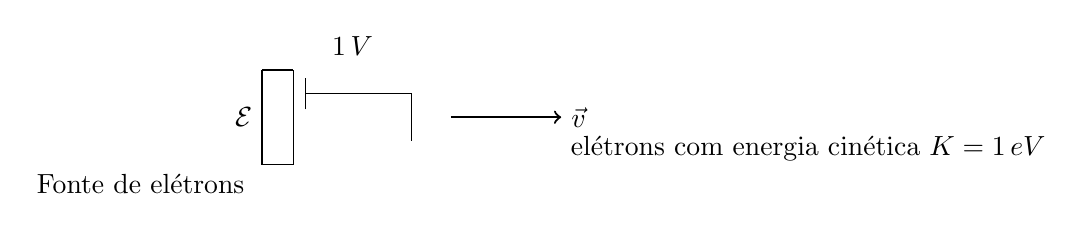
\begin{tikzpicture}[scale=1]
    \draw (0,0) -- (0,0.6);
    \draw (0.15,0.1) -- (0.15,0.5);
    \draw (0,0.6) -- (-0.4,0.6);
    \draw (0.15,0.3) -- (1.5,0.3);
    \draw (1.5,0.3) -- (1.5,-0.3);
    \node at (0.75,0.9) {$1\,\text{V}$};
    \node[left] at (-0.4,0) {$\mathcal{E}$};
    \draw (-0.4,0.6) -- (-0.4,-0.6) -- (0,-0.6) -- (0,0);
    \node[below left] at (-0.5,-0.6) {Fonte de elétrons};
    \draw[->, thick] (2.0,0) -- (3.4,0) node[right] {$\vec{v}$};
    \node[right] at (3.4,-0.4) {elétrons com energia cinética $K = 1\,\text{eV}$};
\end{tikzpicture}
\end{center}

\begin{equation}
    \frac{p^2}{2m} = 1\,\text{eV} \quad \Longrightarrow \quad p = 5{,}4\times10^{-25}\ \text{kg}\cdot\text{m/s}
\label{eq:aula10_p_eletron_1V}
\end{equation}

\begin{equation}
    \lambda = \frac{h}{p} = 12{,}3\ \text{\AA}
\label{eq:aula10_lambda_debroglie_eletron}
\end{equation}

Para ver a interferência, as fendas devem estar \underline{muito} próximas ($d \sim 10\ \text{\AA}$) (para a luz basta $d \sim 5000\ \text{\AA}$).

\begin{center}
\begin{tikzpicture}[scale=0.95]

    \draw[<->] (0.6,2.0) -- (2.6,2.0);
    \node[above] at (1.6,2.1) {$D$};
    \node[left] at (0.0,0.6) {$K=1\text{eV}$};
    \draw[->] (-0.6,0.5) -- (0.0,0.5);
    \draw[->] (-0.6,0.0) -- (0.0,0.0);
    \draw[->] (-0.6,-0.5) -- (0.0,-0.5);
    \draw[thick] (0.6,-1.6) -- (0.6,-0.15);
    \draw[thick] (0.6,0.15) -- (0.6,1.6);
    \draw[<->] (0.3,-0.15) -- (0.3,0.15);
    \node[left] at (0.25,0) {$d$};
    \draw[thick] (2.6,-1.9) -- (2.6,1.9);
    \draw[domain=-1.9:1.9, smooth, variable=\y, samples=100]
        plot ({2.6+0.5*((cos(((\y)*260)))*(exp(-((\y)*(\y))*0.5))}, \y);
    \draw[<->] (3.2,0.15) -- (3.2,1.4);
    \node[right] at (3.4,0.8) {$\dfrac{2D\lambda}{d}$};
    \node[below] at (1.6,-2.2) {$d \sim \lambda \sim 12\ \text{\AA}$};


    \draw[<->] (5.2,2.0) -- (7.2,2.0);
    \node[above] at (6.2,2.1) {$D$};
    \node[left] at (4.6,0.6) {$K=1\text{eV}$};
    \draw[->] (4.0,0.5) -- (4.6,0.5);
    \draw[->] (4.0,0.0) -- (4.6,0.0);
    \draw[->] (4.0,-0.5) -- (4.6,-0.5);
    \draw[thick] (5.2,-1.6) -- (5.2,1.6);
    \draw[thick] (7.2,-1.9) -- (7.2,1.9);
    \draw[domain=-1.9:1.9, smooth, variable=\y, samples=60]
        plot ({7.2+0.55*(exp(-((\y)*(\y))*0.5))}, \y);
    \node[below] at (6.2,-2.2) {$d \gg \lambda$};
\end{tikzpicture}
\end{center}

No caso $d \gg \lambda$, você não consegue perceber as franjas de interferência, que ficam muito juntas.

\textbf{Obs:} Aqui você deve interpretar um máximo de interferência como um ponto do anteparo que recebe muitos elétrons.

\textbf{Obs:} A largura do envelope das franjas de interferência é determinada pela \textbf{LARGURA} dos orifícios, estou supondo que esta permanece a mesma.

As franjas de interferência muito próximas tornam a segunda situação ($d \gg \lambda$) indistinguível de uma distribuição de partículas de acordo com a curva envelope.

\subsection*{O que seria esperado caso os elétrons se movessem como partículas, ao longo de trajetórias?}

\begin{center}
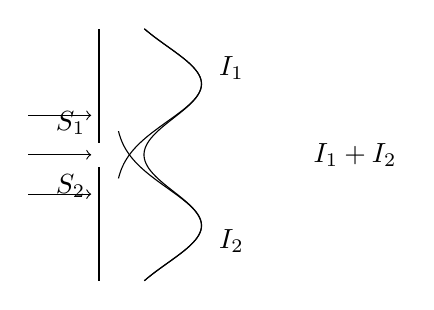
\begin{tikzpicture}[scale=1]
    \draw[thick] (0,-1.6) -- (0,-0.15);
    \draw[thick] (0,0.15) -- (0,1.6);
    \node[left] at (-0.05,0.4) {$S_1$};
    \node[left] at (-0.05,-0.4) {$S_2$};
    \draw[->] (-0.9,0.5) -- (-0.1,0.5);
    \draw[->] (-0.9,0.0) -- (-0.1,0.0);
    \draw[->] (-0.9,-0.5) -- (-0.1,-0.5);

    \draw[domain=-0.3:1.6, smooth, variable=\y, samples=60]
        plot ({0.2+1.1*exp(-((\y-0.9)*(\y-0.9))*2.2)}, \y);
    \node[right] at (1.4,1.1) {$I_1$};

    \draw[domain=-1.6:0.3, smooth, variable=\y, samples=60]
        plot ({0.2+1.1*exp(-((\y+0.9)*(\y+0.9))*2.2)}, \y);
    \node[right] at (1.4,-1.1) {$I_2$};

    \draw[domain=-1.6:1.6, smooth, variable=\y, samples=100]
        plot ({0.2+1.1*exp(-((\y-0.9)*(\y-0.9))*2.2)+1.1*exp(-((\y+0.9)*(\y+0.9))*2.2)}, \y);
    \node[right] at (2.6,0) {$I_1 + I_2$};
\end{tikzpicture}
\end{center}

$I_1$ seria a distribuição das partículas que tivessem passado por $S_1$, e $I_2$ a distribuição das que tivessem passado por $S_2$. Como uma \textbf{PARTÍCULA} (diferente de uma \textbf{ONDA}) não pode passar pelos 2 orifícios, o resultado final deve ser a soma $I_1 + I_2$ (a curva tracejada), que é exatamente o envelope do caso $d \gg \lambda$ acima.

Elétrons e átomos podem exibir interferência e difração, apenas os orifícios e espaçamentos de orifícios devem ser \textbf{MUITO} pequenos. Para orifícios usuais não há como detectar os padrões de interferência, e o resultado pode ser entendido atribuindo-se uma natureza de \textbf{PARTÍCULA} aos elétrons.

No entanto, quando as condições são ajustadas com cuidado, podemos ver interferência e difração \textbf{EMBORA} os elétrons, como os fótons, cheguem ao anteparo como ``pacotes''.

\fbox{\parbox{0.92\textwidth}{
\textbf{Conclusão:} Assim como no caso dos fótons, os elétrons, prótons, átomos, etc., são governados por uma onda que sofre difração e interferência. Essa onda pode ser estudada e seu comportamento previsto (é o que faremos neste curso), mas seu conhecimento não permite prever onde os elétrons, átomos, etc., irão aparecer (exatamente como no caso dos fótons); trata-se de uma \textbf{ONDA DE PROBABILIDADE}! (sem ser muito rigoroso)
}}

\subsection*{Quando devo usar MQ? Ou: quando a natureza ondulatória se manifesta?}

Sempre que a sua ``partícula'' (com licença de linguagem) estiver submetida a uma energia potencial (que reflete o ambiente com o qual ela interage) que varia apreciavelmente na escala de distância de seu comprimento de onda de de Broglie.

\textbf{Exemplo de difração:}

\begin{center}
\begin{tikzpicture}[scale=0.95]

    \draw[<->] (0.6,2.0) -- (2.6,2.0);
    \node[above] at (1.6,2.1) {$D$};
    \draw[->] (-0.6,0.3) -- (0.0,0.3);
    \draw[->] (-0.6,-0.1) -- (0.0,-0.1);
    \draw[->] (-0.6,-0.5) -- (0.0,-0.5);
    \draw[thick] (0.6,-1.6) -- (0.6,-0.15);
    \draw[thick] (0.6,0.15) -- (0.6,1.6);
    \node[left] at (0.5,0) {$a$};
    \draw[<->] (0.6,-0.15) -- (0.6,0.15);
    \draw[thick] (2.6,-1.9) -- (2.6,1.9);
    \draw[domain=-1.9:1.9, smooth, variable=\y, samples=100]
        plot ({2.6+0.5*((cos(((\y)*260)))*(exp(-((\y)*(\y))*0.5))}, \y);
    \draw[<->] (3.2,0.15) -- (3.2,1.4);
    \node[right] at (3.4,0.8) {$\dfrac{2D\lambda}{a}$};
    \node[below] at (1.6,-2.2) {$a \sim \lambda$ (comportamento ONDA)};


    \draw[<->] (5.2,2.0) -- (7.2,2.0);
    \node[above] at (6.2,2.1) {$D$};
    \draw[->] (4.0,0.3) -- (4.6,0.3);
    \draw[->] (4.0,-0.1) -- (4.6,-0.1);
    \draw[->] (4.0,-0.5) -- (4.6,-0.5);
    \draw[thick] (5.2,-1.0) -- (5.2,1.0);
    \node[left] at (5.1,0) {$a$};
    \draw[thick] (7.2,-1.9) -- (7.2,1.9);
    \draw[domain=-1.9:1.9, smooth, variable=\y, samples=60]
        plot ({7.2+0.55*(exp(-((\y)*(\y))*0.5))}, \y);
    \node[below] at (6.2,-2.2) {$a \gg \lambda$ (comportamento PARTÍCULA)};
\end{tikzpicture}
\end{center}
